\subsection{Regular diffusion}
A known inpainting approach is called diffusion. The idea is to fix the known regions of the image and let them diffuse into the unknown regions. This can be done very efficiently by using a convolutional kernel. By iteratively convolving a kernel on the entire image and then restoring the known pixels we can obtain an inpainted image. This process is displayed in figure \ref{fig:diffusion}. The quality of the solution heavily depends on the kernel used. Typically used kernels are the Gaussian kernel and the kernel where all elements are equal (see figure \ref{fig:kernels_1}). A faster is approach is to use these kernel but with the central element set to 0 \cite{richard2001fast} (see figure \ref{fig:kernels_2}).

\begin{figure*}[h]
	\centering
	\begin{subfigure}[b]{0.47\textwidth}
		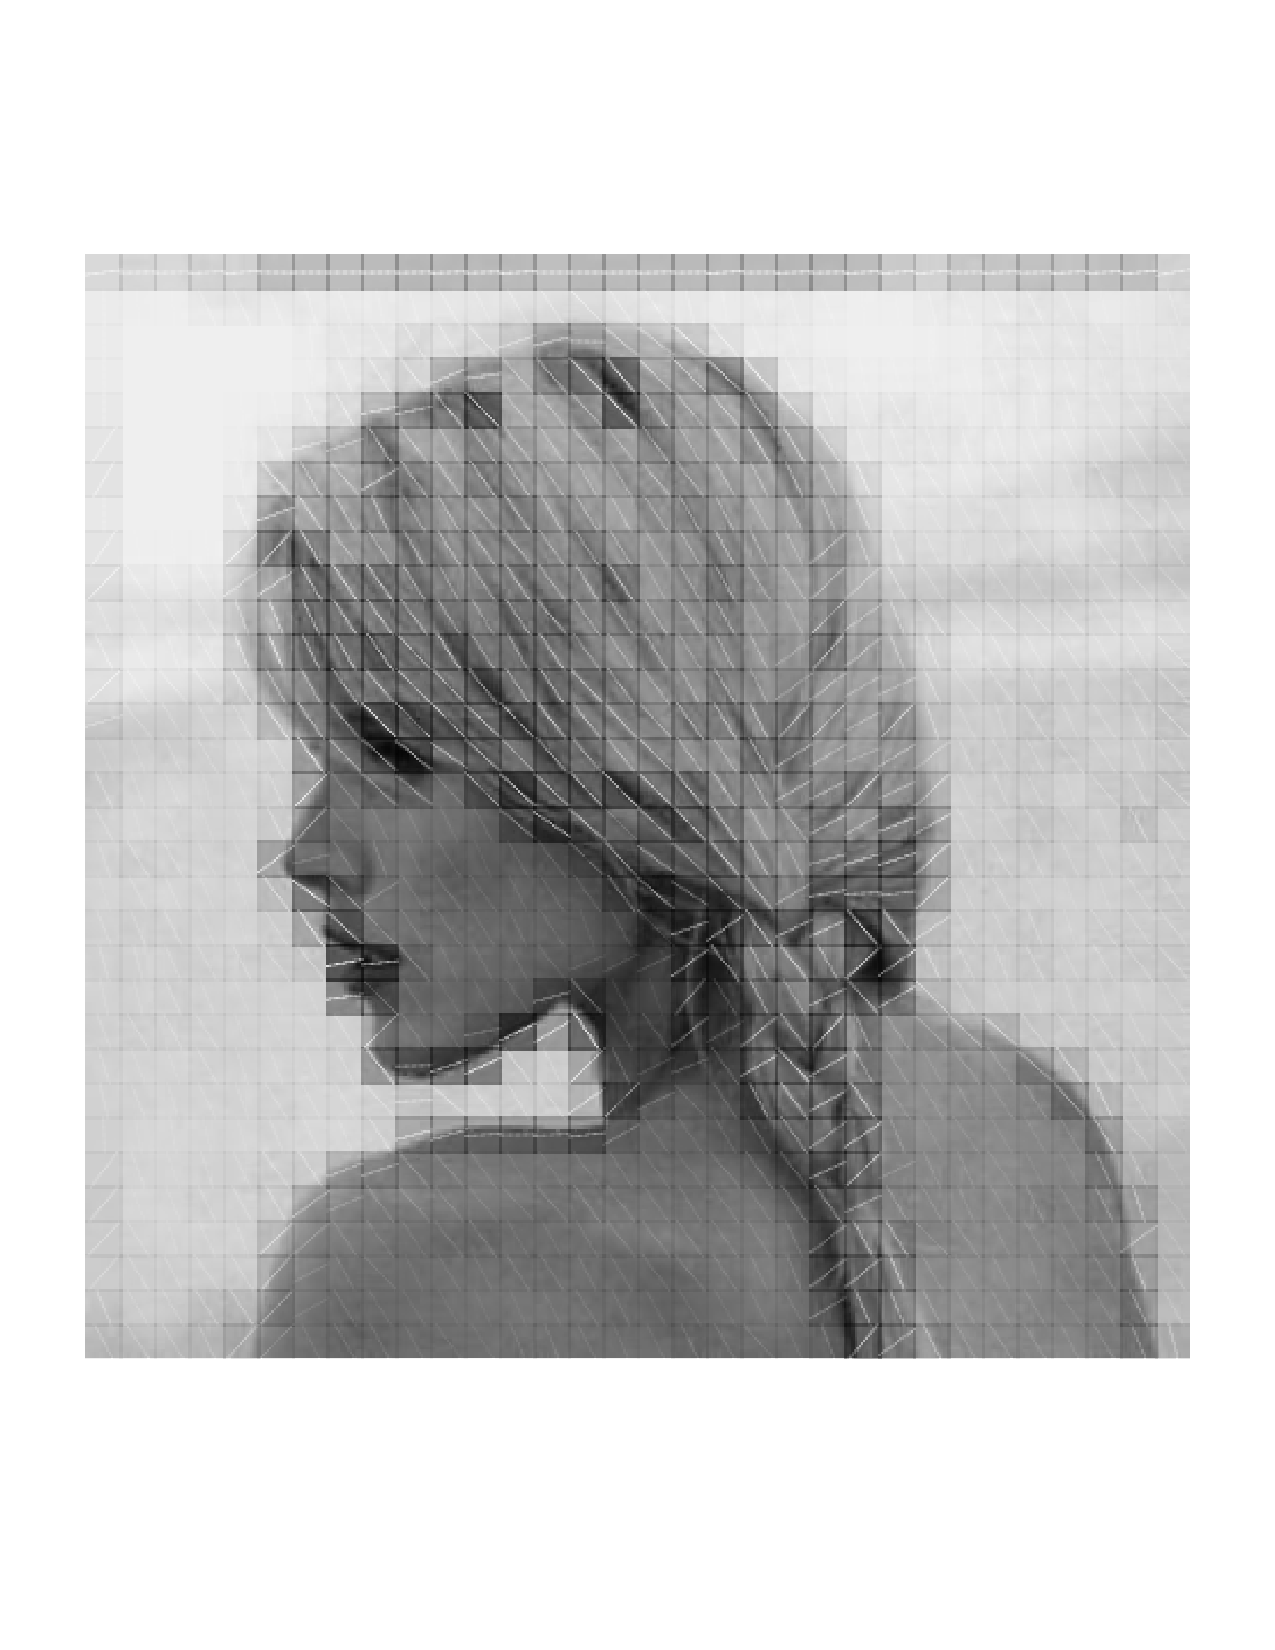
\includegraphics[trim=2cm 5cm 2cm 5cm, clip=true, width=\textwidth]{figures/directional_claudia}
		\caption{The claudia image.}
		\label{fig:claudia}
	\end{subfigure}
	\begin{subfigure}[b]{0.47\textwidth}
		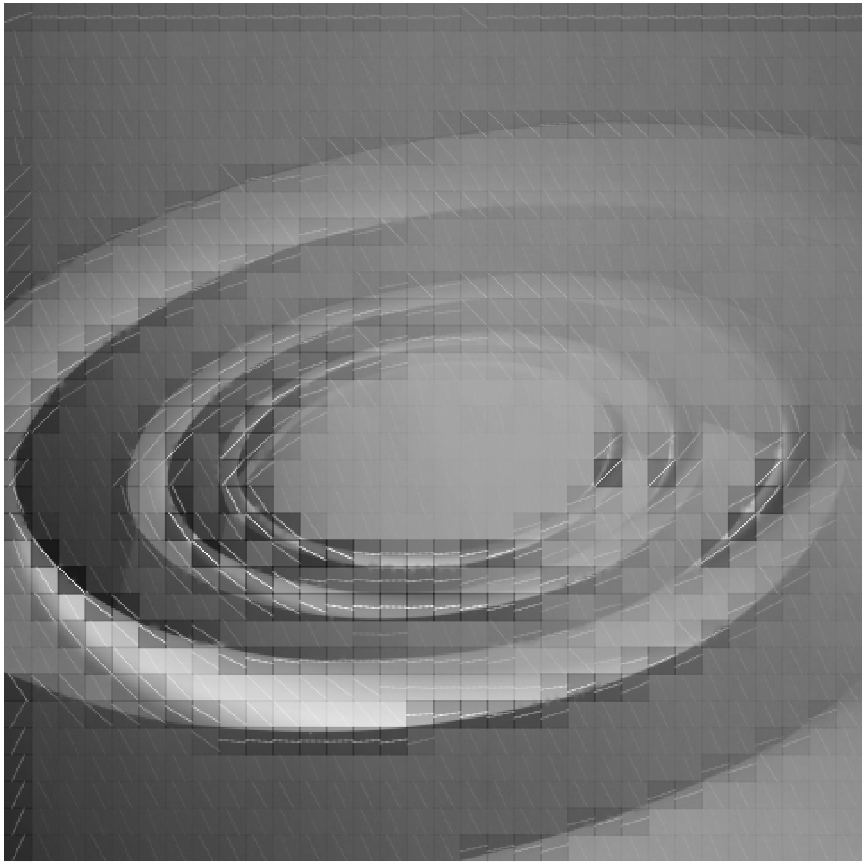
\includegraphics[trim=2cm 5cm 2cm 5cm, clip=true, width=\textwidth]{figures/directional_spiral}
		\caption{The spiral image.}
		\label{fig:spiral}
	\end{subfigure}

	\caption{The directionality of 16x16 patches shown as white lines. The relative darkness of each patch shows the contrast of the underlying image and will contain more pronounced edges.}
	\label{fig:directionality}
\end{figure*}